\section{Modèles théoriques}\label{sec:rw:sgfd:modeles}
Nous avons présenté brièvement dans le chapitre~\ref{chap:rw:supervision} que les systèmes de gestions de flux de données s'inspiraient du modèle relationnel. Le modèle relationnel ne supporte toutefois pas le dynamisme des données. Ainsi de nombreuses propositions ont été faites dans l'état de l'art pour reconstruire un modèle tout en tentant de réutiliser les connaissances développées sur les systèmes de gestion de base de données relationnels depuis 40 ans.

Dans cette section, nous allons détailler l'historique de la recherche dans ce domaine. Pouvoir observer l'évolution des modèles au fur et à mesure des années permet en effet de bien cerner les problématiques théoriques lié à la gestion de flux. En~\ref{sec:rw:sgfd:modeles:early}, nous présenterons l'établissement des premiers modèles. En~\ref{sec:rw:sgfd:modeles:stream}, nous présenterons la sémantique abstraite mélangeant flux et relations. Puis nous présenterons en~\ref{sec:rw:sgfd:modeles:batch} les initiatives de clarifications et reformalisation des modèles existants. Enfin, nous présenterons une synthèse de ces travaux.

\subsection{La genèse de la gestion de flux}\label{sec:rw:sgfd:modeles:early}
L'idée de créer des requêtes continues a été présenté en 1992 dans le système Tapestry~\cite{Terry:tapestry}. Dans ce système une requête continue est avant tout une requête instantanée, mais la sémantique étant que celle-ci sera exécuté périodiquement. Ces requêtes s'appliquent sur un ensemble de données sans suppression ou mise à jour (\textit{append-only}). Le résultat de cette requête sera représenté par le flux des nouvelles données calculés de manière incrémental. Pour cela, les relations sont réellement considérés comme des variables et elles deviennent donc dépendantes du temps.

En 1995, les flux de données ont été explorés tout d'abord par le modèle séquentiel $\mathcal{SEQ}$~\cite{Seshadri:seq}. Dans ce modèle, une \enquote{\it séquence} est un ensemble d'enregistrements (n-uplets relationnels) avec un ordre positionnel. Dans le modèle relationnel originel~\cite{Codd:model}, ceci n'est pas autorisé car l'ordre des n-uplets est dit \enquote{\it irrelevant}. La sémantique de spécification des opérateurs relationnels utilise cet liberté d'ordre pour être consistent et obtenir des propriétés intéressantes (voir chapitre~\ref{chap:contrib:astral}). Ici, le formalisme de $\mathcal{SEQ}$ montre qu'il est toujours possible d'exploiter les opérateurs algébriques classiques et que de nouveaux peuvent être créés comme les premières notions de regroupements d'n-uplets appelées \textit{collapse}\footnote{Cette primitive représente ce qui deviendra l'opérateur de fenêtrage plus tard}. Ce formalisme a été fondateur pour plusieurs travaux futurs qui s'inspirent explicitement de ce modèle~\cite{Gurgen:sens,Babcock:issues}.

Par la suite, les premières opérations sur les flux en tant que tels ont pu apparaître avec le système Chronicle~\cite{Jagadish:chronicle}. Toutefois, les flux étaient considérés soit comme un ensemble de données historique, soit comme une données constamment mise à jour (fenêtres complète, ou instantanée). La notion de fenêtre a été présenté pour la première fois dans Tribeca~\cite{Sullivan:tribeca,Sullivan:tribeca2}. Sa spécification était basée sur sa taille positionnelle (nombre de données) ou temporelle (durée). Toutefois, ce système ne pouvait gérer qu'un seul flux à la fois. La notion de fenêtre sera par la suite intégrée à SQL:1999~\cite{Melton:sql1999} ainsi que dans SQL:2003~\cite{Eisenberg:sql2003} pour des opérations OLAP.

Les requêtes continues ont été aussi développés grâce aux besoins de plus en plus demandant des bases de données en constante évolution. Lors de la fin de années 90, les bases de données contenant des pages et flux web dynamiques ont de graves problèmes de performances pour analyser les flux d'événements. Ceci débouchera sur des projets tels que OpenCQ~\cite{Liu:opencq} et surtout NiagaraCQ~\cite{Chen:niagaracq} qui permettent de faire notamment des opérations de jointures.

Le début des années 2000 a marqué l'avènement des systèmes de gestion de flux de données à part entière. Cela a notamment été motivé par l'arrivée d'applications réseaux~\cite{Cranor:gigascope} et capteurs~\cite{Madden:tag,Yao:cougar} demandeurs de plus en plus de puissance d'expression ainsi que de performances. A quelques mois d'intervalles, les premiers SGFD ont donc fait leur apparition : TelegraphCQ~\cite{Chandrasekaran:telegraphcq} et Aurora~\cite{Carney:monitoring} et STREAM~\cite{Widom:queries}. Ce dernier apporte de plus son algèbre : SQuAl~\cite{Abadi:aurora}. Celle-ci sera la première algèbre complète sur les flux de données. Un flux est considéré comme un ensemble de n-uplets strictement ordonnés avec un schéma prédéfinit $(\textbf{TS}, A_1,\dots, A_n)$, où $\textbf{TS}$ correspond au \textit{timestamp}. L'algèbre décrit le comportement d'opérateurs simples comme la sélection (\textit{Filter}), la projection-évaluation (\textit{Map}) et l'union (\textit{Union}). Mais aussi d'opérateurs complexes (i.e. utilisant une fenêtre) tels que le tri à la volée (\textit{BSort}), l'agrégat (\textit{Aggregate}), la jointure sur bande (\textit{Join}) et un opérateur de synchronisation de \textit{timestamp} (\textit{Resample}). Il est important de voir que ces opérateurs complexes se définissent grâce à des fenêtres prédéfinies à l'avance. 

TelegraphCQ~\cite{Chandrasekaran:telegraphcq} quant à lui proposait un langage de requête beaucoup plus axé sur le relationnel avec notamment une définition de fenêtre générique. En effet ces dernières étaient décrites par une séquence de type \textit{boucle for}.
\begin{center}
\begin{minipage}[c]{0.75\textwidth}
\begin{verbatim}
for(t=initial_value; continue_condition(t); change(t)) {
    WindowIs(StreamA, left_end(t), right_end(t));
    WindowIs(StreamB, left_end(t), right_end(t)); …
}
\end{verbatim}
\end{minipage}
\end{center}

Cependant, depuis le début des requêtes continues, la spécification des opérateurs étaient avant tout dirigés par l'implémentation. Cela a amené a des limitations d'expressivité (voire même des divergences d'interprétation). Ceci a été notamment traité dans le SGFD générique STREAM.

\subsection{La sémantique abstraite à deux concepts}\label{sec:rw:sgfd:modeles:stream}
Le système STREAM~\cite{Widom:queries, Arasu:stream} se démarque des autres systèmes de son époque pour avoir décrit une sémantique abstraite à deux concepts~\cite{Arasu:semantic} :
\begin{itemize}
 \item[\textbf{Un flux}] est un ensemble potentiellement infini d'n-uplets conformes à un schéma commun possédant un \textit{timestamp}.
 \item[\textbf{Une relation}] Une relation est une fonction qui associe le temps à un ensemble fini d'n-uplets conformes à un schéma commun.
\end{itemize}
Le point crucial de cette approche est le fait que les opérateurs sont capables de passer d'un concept à l'autre (voir figure~\ref{fig:rw:sgfd:streamrelation}. Ainsi, les opérateurs capables de traiter des relations pour en fournir une nouvelle sont les opérateurs relationnels. Ceux-ci sont notamment issus de l'algèbre relationnelle usuelle (réadapté pour être conforme formellement au modèle évidemment) tels que $\sigma$, $\Pi$ et même $\Join$. Les opérateurs transformant un flux en relation sont les opérateurs de fenêtres. Les opérateurs transformants les flux en relations sont des \textit{streamers}.
\begin{figure}[ht]
    \centering
    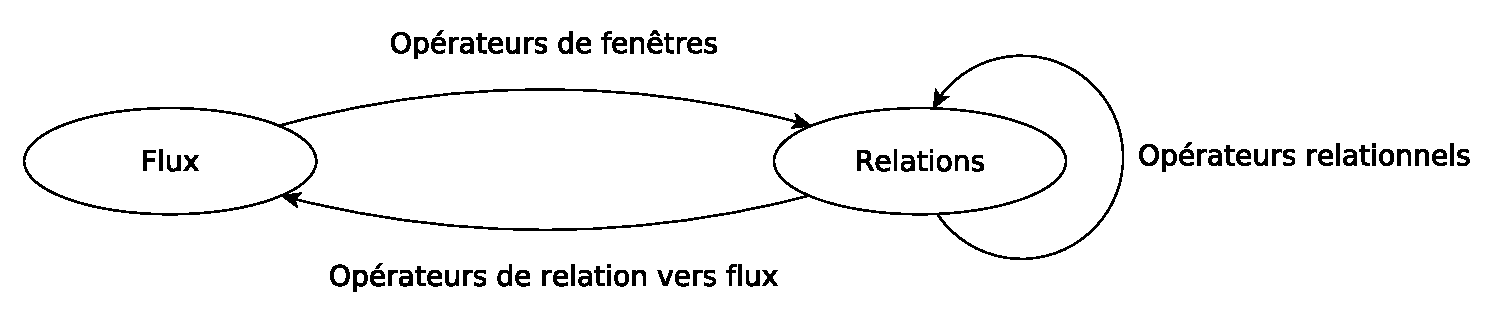
\includegraphics[width=0.75\textwidth]{rw-sgfd-streamrelation}
    \caption{Associations utilisés dans la sémantique abstraite de STREAM}\label{fig:rw:sgfd:streamrelation}
\end{figure}

Afin de mieux illustrer la sémantique abstraite utilisée, nous allons détailler un exemple plus concrêt.
\begin{example}
Soit $S$ un flux de capteurs $(\mathrm{temperature}, \textbf{T})$ avec \textbf{T} pour \textit{timestamp} et temperature pour sa mesure. Nous souhaitons faire un agrégat sur 5 min. La composition d'opérateur sera la suivante :
\begin{itemize}
\item D'abord un opérateur de fenêtrage $[5min]$ sera appliqué. Il transformera le flux en la relation \textit{groupement des 5 dernières minutes}. Cette relation évolue évidemment au cours du temps.
\item Ensuite un opérateur d'agrégation\footnote{notation simplifiée de l'opérateur d'agrégation sans groupement dont le résultat est une relation avec un seul attribut \textit{avg}} $\mathcal G_{avg(temp)}$. Nous obtenons ainsi une relation avec un seul n-uplet.
\item Enfin, un opérateur de \textit{streaming} est appliqué. Celui-ci peut avoir plusieurs sémantique. Prenons le plus simple $ISTREAM$ qui permet de créer un flux à partir des insertions dans la relation (une mise à jour est considéré comme une suppression puis insertion).
\end{itemize}
Nous aurons donc au final la requête suivante : $$ISTREAM(\mathcal G_{avg(temp)}(S[5min]))$$
\end{example}

Le point clé et novateur de cette approche étant que les opérateurs de flux vers flux \textbf{n'existe pas}. Ce point est important car jusqu'à présent tous les opérateurs étaient de cette forme. Par exemple, la jointure de deux flux n'existe pas par essence. Seule la jointure de relations est possible, et il est possible de créer des relations à partir de fenêtrages sur flux. Les auteurs ont justifié cette approche car l'écriture de requête était plus intuitive et que cela permettait de généraliser l'utilisation des vues matérialisés dans le traitement des flux (introduit auparavant dans Chronicle). La spécification de cette sémantique a permit par la suite de décrire le langage associé CQL~\cite{Arasu:cql} (\textit{Continuous Query Language}) dérivé du \textit{SQL} qui est désormais utilisé dans de nombreux produits académiques et commerciaux~\cite{Witkowski:oraclecq,url:sqlstream}.

\begin{example}
La requête \textit{CQL} de l'exemple précédent aura la forme suivante : 
\begin{center}
\it ISTREAM(SELECT AVG(temp) as avg FROM S [RANGE 5min])
\end{center}
\end{example}

La sémantique formelle du langage CQL est présenté au complet dans la thèse d'Arvind Arasu~\cite{Arasu:queries}. L'algèbre \textit{ACO} (\textit{Algebra of Continuous Operators}) y est décrite. Les définitions élémentaires sont les suivantes : 
\begin{itemize}
 \item[\textbf{Instant} ($\tau$)] : élément de l'ensemble $\mathcal T$, discret et ordonné\footnote{Il est en réalité définit comme un ensemble satisfaisant les axiomes de Peano. En particulier la présence d'un unique successeur. L'instant de départ de l'exécution est le plus petit instant observé, donc $0$.} et représenté par $\N$.
 \item[\textbf{Relation}] : Fonction associant un instant à un multi-ensemble de n-uplets avec un schéma commun.
 \item[\textbf{Flux}] : Multi-ensemble d'éléments $\left<s,\tau\right>$ où $s$ est un n-uplet respectant un schéma commun et $\tau \in \mathcal T$ son \textit{timestamp}. Pour un $\tau$ donné, il doit y avoir un nombre fini (mais non borné) d'éléments.
\end{itemize}
Par la suite, il est possible de définir des opérateurs sur ces éléments. Les opérateurs relationnels sont simple car pour une \textit{relation} $R$, et un instant $\tau$ : la \textit{relation instantanée} $R(\tau)$ est une relation au sens SGBD du terme\footnote{D'un point de vue strict, les multi-ensembles sont utilisés dans les SGBD mais ne sont pas originellement utilisé dans le modèle relationnel.}. Il est donc possible d'y appliquer les opérateurs classiques. Ainsi nous avons les équivalences suivante : $\forall \tau\in\mathcal T,$ 
\begin{eqnarray*}
    (\sigma_c R)(\tau) & = & \sigma_c(R(\tau))\\
    (R_1 \Join R_2)(\tau) & = & R_1(\tau) \Join R_2(\tau)
\end{eqnarray*}

Les opérateurs les plus importants sont ceux de classe $S2R$ (\textit{stream-to-relation}) et $R2S$ (\textit{relation-to-stream}). La table~\ref{tab:rw:sgfd:acostream} liste les opérateurs présentés.
 
\begin{table}[ht]
 \centering
\begin{tabular}{|c|c|l|}\bottomrule
Opérateur & Classe & Description \\\toprule \bottomrule
$S[N]$ & $S2R$ & Fenêtre positionnelle glissante de taille $N$ n-uplets \\ \hline
$S[W]_T$ & $S2R$ & Fenêtre temporelle glissante de taille $W$ unités de temps \\\hline
$S[1]_T$ & $S2R$ & Fenêtre représentant l'instant présent\\\hline
$S[\infty]$ & $S2R$ & Fenêtre accumulative\\ \toprule \bottomrule
$\mathcal{IS}(R)$ & $R2S$ & Flux d'insertion \\ \hline
$\mathcal{DS}(R)$ & $R2S$ & Flux de suppression \\ \hline
$\mathcal{RS}(R)$ & $R2S$ & Flux de présence \\ \toprule
\end{tabular}
\caption{Opérateurs de flux de l'algèbre \textit{ACO}}\label{tab:rw:sgfd:acostream}
\end{table}

Pour les \textit{streamers}, leurs définitions sont dérivées de l'état de la relation à l'instant présent ainsi que à l'instant précédent. Leurs définitions sont donc dépendant de la discrétisation du temps. Soit $R$ une relation, 
\begin{eqnarray*}
    \mathcal{IS}(R) & = & \bigcup_{\tau\geq 0} ((R(\tau) - R(\tau-1))\times \{\tau\})\\
    \mathcal{DS}(R) & = & \bigcup_{\tau>0} ((R(\tau-1) - R(\tau))\times \{\tau\})\\
    \mathcal{RS}(R) & = & \bigcup_{\tau\geq 0} (R(\tau)\times \{\tau\})
\end{eqnarray*}
La définition des fenêtres est quant à elle plus technique. L'idée étant de regrouper les n-uplets selon un critère particulier. Soit $S$ un flux,
\begin{eqnarray*}
    S[W]_T & = & \left\{s | \left<s,\tau'\right>\in S \wedge (\tau' \leq \tau) \wedge (\tau' \geq \max\{\tau - W +1,0\})   \right\}\\
    S[N] & = & \left\{s_i \in S | \max\{1,n(\tau)-N+1\} \leq i \leq n(\tau)\right\}
\end{eqnarray*}
où la suite $(s_n)$ correspond à la suite des n-uplets ordonnées par \textit{timestamp} et $n(\tau)$ le nombre d'éléments de $S$ possédant un \textit{timestamp} $\leq \tau$.

Le langage \textit{CQL} et cette algèbre \textit{ACO} ont été démontré comme plus expressifs~\cite{Arasu:cql} que les autres solutions que nous avons mentionné précédemment (Chronicles, Tribeca, Tapestry, Gigascope, Aurora et TelegraphCQ).

\subsection{La reformalisation}\label{sec:rw:sgfd:modeles:batch}
À partir de 2005, plusieurs travaux se sont intéressé à la formalisation stricte de la sémantique des opérateurs. Le plus étudié reste l'opérateur de fenêtrage qui est une des principales raisons de la complexité des systèmes de gestion de flux de données~\cite{Maier:semantics,Patroumpas:window,Patroumpas:subsumewindows}. Les conséquences d'une meilleure compréhension de cet opérateur sont certains sur l'interprétation de sa sémantique complexe de son fonctionnement mais aussi pour permettre des procédés d'optimisations tels que le partage de résultats (voir section~\ref{sec:rw:sgfd:optim}).

En 2008, les auteurs à l'origine de \textit{STREAM}, d'\textit{Aurora}, de \textit{StreamBase} et d'\textit{Oracle CQ} ont présenté~\cite{Jain:spread} pour dénoncer l'ambiguïté sémantique des langages de gestion de flux. En effet, l'exécution des opérateurs complexes tels que les fenêtres n'étaient pas identique entre l'interprétation de \textit{StreamBase} et l'interprétation d'\textit{Oracle}. Le point clé étant le modèle d'exécution. Afin d'illustrer le phénomène, voici un exemple.

\begin{example}\label{ex:rw:sgfd:batches}
 Soit $S$ un flux dont le contenu est, dans le formalisme \textit{ACO}, $\{\left<s_1,0\right>, \left<s_2,0\right>, \left<s_3,1\right>\}$. Nous souhaitons observer le résultat de la requête $S[1]$ (fenêtre de 1-tuple).

Si le modèle d'exécution est basé sur l'arrivée des n-uplets. Alors lorsque le n-uplet $s_1$ entre dans le système. Le système remplit une nouvelle fenêtre, ce qui donne $S[1](0)=\{s_1\}$. Puis viens le n-uplet $s_2$ et le système produit une nouvelle fenêtre : $S[1](0)=\{s_2\}$. L'avantage étant que les n-uplets sont tous considérés, toutefois au même instant, la fenêtre a deux états différents, ce qui n'est pas correct.

Si le modèle d'exécution est basé sur les \textit{timestamps}. Alors à l'instant 0, l'opérateur va obtenir les deux n-uplets. Puis, conformément à sa spécification algébrique, va sélectionner l'un d'eux, pour produire $S[1](0) = \{s_1\}$ ou $\{s_2\}$. Le point de vue formel est cette fois correct, toutefois cet opérateur va perdre des données, ce qui peut être problématique.
\end{example}

Le problème étant que les deux sémantiques ont du sens a priori. Pour clarifier, les auteurs introduisent la notion de \textit{batch}. La figure~\ref{fig:rw:sgfd:modes} présente les différents modes d'exécutions. Le mode basé sur le temps groupe tous les n-uplets qui possèdent le même \textit{timestamp}. Le mode basé sur les n-uplets au contraire se base sur chaque n-uplet. Le batch est une généralisation de ces modes puisqu'il considère que l'ensemble des n-uplets simultanés est partitionné en un sous ensemble ordonné.
\begin{figure}[ht]
    \centering
    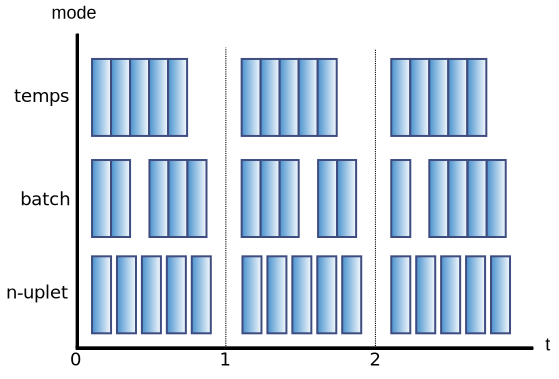
\includegraphics[width=0.75\textwidth]{rw-sgfd-modes}
    \caption{Représentation des différents modes d'exécution des SGFD}\label{fig:rw:sgfd:modes}
\end{figure}
L'unité de temps n'est donc pas le \textit{timestamp} ou l'n-uplet, ce sont les batchs. D'un point de vue physique, cela correspond à un \textit{envoi groupé} de la part de la source.
\begin{example}
 Une source d'événement produit un flux d'information. Si deux événements se produisent au même \textit{instant} (à l'unité de temps près)\footnote{Ces cas apparaissent facilement dans les cadres de grande échelle ou lorsqu'un événement est cause d'un autre}, la source effectuera quand même deux actions de production de la source, ces productions correspondent aux batchs.
\end{example}

Par la suite, des opérateurs sont développés pour manipuler les batchs pour passer d'un mode d'exécution à l'autre. Par exemple, il est possible de structurer les batchs d'un \textit{timestamp} donné à partir d'un autre attribut (identifiant par exemple).

De façon similaire, nous pouvons effectivement remarquer que dans l'algèbre \textit{ACO} la gestion de l'ordre positionnel est flou Le flux est ordonné par \textit{timestamp}, mais en cas de n-uplets dits \textit{simultanés}, aucun ordre strict n'est définit. Dans la définition de la fenêtre positionnelle, \textit{ACO} introduit la définition d'une suite $(s_n)$ strictement ordonnée. A. Arasu a dit sur ce point dans son manuscrit de thèse : \enquote{\it Comme nous ordonnons arbitrairement la séquence $s_1$, $s_2$,..., les fenêtres positionnelles sont non-déterministes lorsque les \textit{timestamps} ne sont pas uniques, ce qui peut ne pas être approprié}. L'introduction apporte donc une généralisation de l'ordre temporel, ce qui peut permettre d'empêcher certains cas. Toutefois, s'il est nécessaire de sélectionner un nombre limité comme dans l'exemple~\ref{ex:rw:sgfd:batches}, le choix reste non-déterministe.

Suite à l'identification des problèmes de modes d'exécution, le modèle \textit{SECRET} a été développé. Le principe étant de décomposer l'opérateur de fenêtre en trois parties. Tout d'abord, le modèle décrit sa portée et son contenu (\textit{scope \& content}) pour savoir quels n-uplets seront inclus dans les fenêtres. Ensuite, les auteurs détaillent son mode de consommation d'n-uplet (\textit{tick}), et enfin son mode de notification à l'utilisateur. Cette séparation claire des concepts permet d'avoir une meilleur compréhension des sémantiques possibles sur les fenêtres. Ainsi, ce modèle permet de décrire les modes de fonctionnement de systèmes existants pour mieux permettre leur intégration par la suite.

Enfin, les travaux de Krämer~\cite{Kramer:semantics} détaillent une algèbre de manipulation des flux, le point novateur étant le fait de séparer l'aspect brut, logique et physique. Les flux tels que nous les avons décrit dans cette section sont des flux bruts composés de couples $(\textrm{n-uplet},\textit{timestamp})$. Les flux logiques sont quant à eux un ensemble de triplets $(\textrm{n-uplet}, \textit{timestamp}, n)$. La multiplicité $n$ permet de compter le nombre d'occurrences du n-uplet a été observée dans le flux originel. Les flux physiques utilisent eux une définition très similaire à ce qui peut se trouver dans les bases de données temporelle avec un intervalle de validité. Ses élements sont donc des couples $(\textrm{n-uplet},[t_s, t_e[)$. Deux algèbres sont ainsi décrites, l'une pour les flux logiques (manipulés pour la sémantique) et l'autre pour les flux physiques (manipulés par l'implémentation). Des équivalences d'expressions sont ensuite définies pour manipuler ces notions.

\subsection{Synthèse}
Beaucoup de modèles théoriques ont été spécifiés lors de ces 15 dernières années pour gérer les flux de données. La sémantique est de plus en plus claire pour la plupart des opérateurs même complexes. Les premiers résultats d'équivalences de requêtes ont pu voir le jour. Toutefois, certains points sont encore manquants :
\begin{itemize}
 \item[\textbf{Le fenêtrage}] : malgré les efforts récurrents de formalisation de cet opérateur, la sémantique reste souvent restreinte à la fenêtre glissante. Qu'en est-il des fenêtres moins conventionnelles mélangeant à la fois les positions et le temps ? Ce type de fenêtre apparait pourtant dans des systèmes d'observations \textit{fenêtre sur 5 données, toutes les 3 minutes}.
 \item[\textbf{L'ordre}] : comme nous l'avons présenté, certains traitement considèrent que des résultats peuvent être non-déterministe. Cet aspect montre un caractère aléatoire qui peut ne pas être de rigueur. Quels sont les conséquences si des ordres plus stricts sont imposés ?
 \item[\textbf{La synchronisation}] : les algèbres manipulent une requête avec un \textit{timestamp} de départ $t_0$. Si ce \textit{timestamp} est altéré la sémantique finale ne sera pas la même, rendant ainsi le partage des résultats plus délicat.
 \item[\textbf{Les équivalences}] : plusieurs équivalences de requêtes simple existent déjà. Toutefois, elles sont souvent remises en question avec des modèles plus expressifs. Comme les équivalences de requêtes sont la pierre angulaire pour permettre une optimisation logique, il est nécessaire d'investiguer sur ce point.
 \item[\textbf{Le couplage relationnel}] : il a toujours été supposé possible de faire des jointures avec des \textit{relations statiques} dans les algèbres. Toutefois, les relations issues d'SGBD ne sont pas statiques dans le temps. La prise en compte des mises à jours dans le modèle est crucial pour permettre d'effectuer le couplage SGBD-SGFD que nous avons mentionné en conclusion du chapitre~\ref{chap:rw:supervision}.
\end{itemize}

